\chapter{Pilas electroquímicas y electrólisis}\label{ch:g12:cells-and-electrolysis}

Un teléfono marca un 1 \% una tarde de invierno y se apaga. Enchufado
durante la noche, por la mañana vuelve a estar lleno. Dentro de su
batería, la misma \omterm{def:g7:chemical-reactions:reaction}{reacción química} funciona en un sentido durante el
día, liberando energía eléctrica, y el cargador la obliga a ir en el otro
sentido por la noche. Una \omterm{def:g11:redox:reaction}{reacción redox} se convierte en una fuente de
electricidad cuando se obliga a sus \omterm{def:g9:inside-the-atom:nucleus}{electrones} a viajar por un cable; y
la electricidad, empujada a través de una disolución, puede forzar una
\omterm{def:g11:redox:reaction}{reacción redox} que nunca ocurriría por sí sola.

\begin{recall}
Los \omterm{def:g11:redox:oxidant}{oxidantes} ganan \omterm{def:g9:inside-the-atom:nucleus}{electrones} y los \omterm{def:g11:redox:oxidant}{reductores} los pierden;
\omterm{def:g11:redox:couple}{semiecuaciones}, \omterm{def:g11:redox:couple}{pares redox} y \omterm{def:g11:redox:reaction}{reacciones redox} (\cref{ch:g11:redox}). Un
sistema evoluciona hasta que $Q = K$ (\cref{ch:g12:equilibrium}). Las
disoluciones de \omterm{def:g9:ions:ion}{iones} conducen la electricidad (\cref{ch:g9:ions}); el
\omterm{def:g10:the-mole:amount}{mol} y la \omterm{def:g10:the-mole:avogadro}{constante de Avogadro}
(\cref{ch:g10:the-mole}).
\end{recall}

\begin{omfigure}
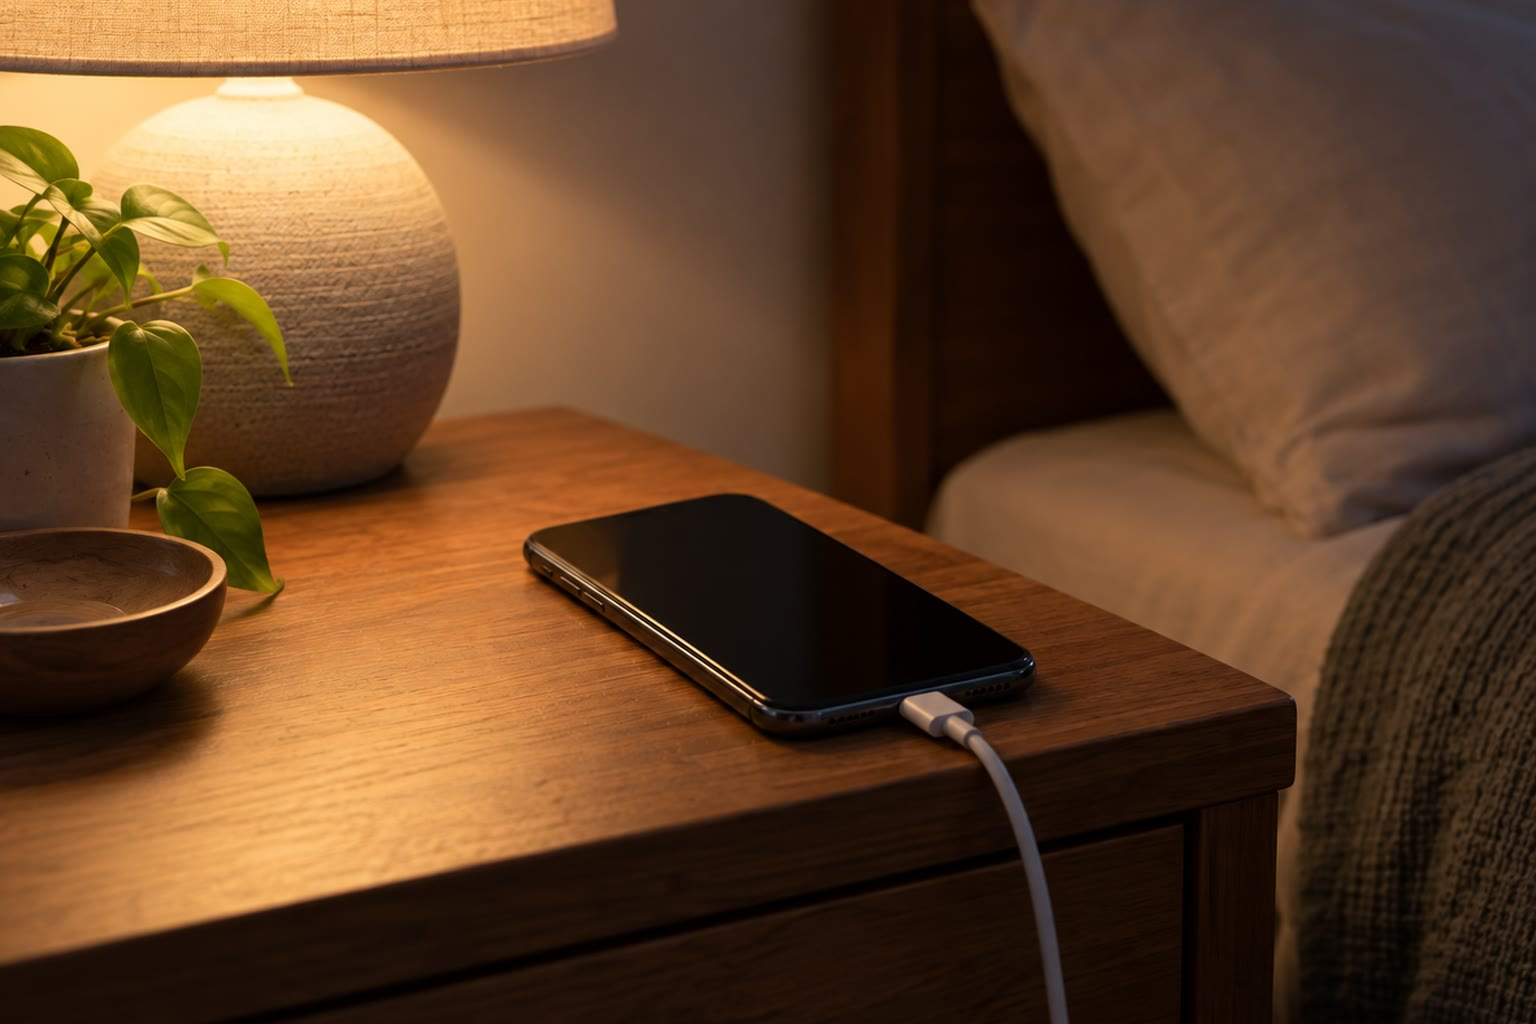
\includegraphics[width=0.45\linewidth]{images/book1/ai/g12-phone-charging.jpg}

{\small Cargar un teléfono: una reacción forzada en sentido inverso
durante la noche.}
\end{omfigure}

\section{Una reacción redox partida en dos}

Cuando se sumerge una lámina de cinc en una disolución de sulfato de
cobre, el cinc se oxida y los \omterm{def:g9:ions:ion}{iones} cobre se reducen en la superficie de
la lámina, \ce{Zn + Cu^{2+} -> Zn^{2+} + Cu}: los \omterm{def:g9:inside-the-atom:nucleus}{electrones} pasan
directamente del \omterm{def:g9:periodic-table-first-look:metal}{metal} a los \omterm{def:g9:ions:ion}{iones}, y la energía se pierde en forma de un
poco de calor. Si se separan las dos mitades y se unen con un cable, los
\omterm{def:g9:inside-the-atom:nucleus}{electrones} tienen que viajar ahora por el cable, y pueden encender una
lámpara por el camino.

\begin{definition}[Pila electroquímica, semipila, puente salino]\label{def:g12:cells-and-electrolysis:cell}
Una \emph{pila electroquímica}\index{pila electroquimica@pila electroquímica} produce
energía eléctrica a partir de una \omterm{def:g11:redox:reaction}{reacción redox} cuya \omterm{def:g11:redox:oxidation}{oxidación} y cuya
\omterm{def:g11:redox:oxidation}{reducción} tienen lugar en dos compartimentos separados. Cada
compartimento, un electrodo metálico sumergido en una disolución de sus
\omterm{def:g9:ions:ion}{iones}, es una \emph{semipila}\index{semipila}. Un \emph{puente
salino}\index{puente salino}, un tubo o una tira de papel empapada en una
disolución de \omterm{def:g9:ions:ion}{iones}, une las dos disoluciones y cierra el circuito sin
dejar que se mezclen.
\end{definition}

\begin{definition}[Ánodo, cátodo]\label{def:g12:cells-and-electrolysis:anode}
El electrodo donde tiene lugar una \omterm{def:g11:redox:oxidation}{oxidación} es el
\emph{ánodo}\index{anodo@ánodo}; el electrodo donde tiene lugar una \omterm{def:g11:redox:oxidation}{reducción}
es el \emph{cátodo}\index{catodo@cátodo}.
\end{definition}

\begin{omfigure}
\begin{tikzpicture}[font=\small, scale=1.25]
  \pic[transform shape] at (0,0) {beaker={0.7}{black!6}};
  \pic[transform shape] at (4,0) {beaker={0.7}{cyan!70!blue!35}};
  \pic[transform shape] (zn) at (-0.3,0.25) {electrode={black!30}};
  \pic[transform shape] (cu) at (4.3,0.25) {electrode={orange!70!brown}};
  \pic[transform shape] at (0.35,0.6) {saltbridge={3.3}};
  \pic[transform shape] (v) at (2,3.9) {meter={1.10 V}};
  \draw[black!70, thick] (zn-top) |- (1.0,3.4) -| (v-a);
  \draw[black!70, thick] (cu-top) |- (3.0,3.4) -| (v-b);
  \draw[->, omProp, very thick] (0.2,3.55) -- (1.0,3.55);
  \draw[->, omProp, very thick] (3.0,3.55) -- (3.8,3.55);
  \node[omProp, font=\footnotesize] at (0.6,3.75) {$e^-$};
  \node[omProp, font=\footnotesize] at (3.4,3.75) {$e^-$};
  \node[anchor=north, align=center] at (-0.2,-0.15) {ánodo ($-$): cinc\\ \ce{Zn -> Zn^{2+} + 2e-}};
  \node[anchor=north, align=center] at (4.2,-0.15) {cátodo ($+$): cobre\\ \ce{Cu^{2+} + 2e- -> Cu}};
  \node[font=\footnotesize, anchor=east, align=right] at (-0.95,0.7) {\ce{Zn^{2+}}\\ \ce{SO4^{2-}}};
  \node[font=\footnotesize, anchor=west, align=left] at (4.95,0.7) {\ce{Cu^{2+}}\\ \ce{SO4^{2-}}};
  \node[font=\footnotesize, align=center] at (2,2.45) {puente salino\\ (\ce{K+}, \ce{NO3-})};
\end{tikzpicture}

{\small La pila Daniell. Los \omterm{def:g9:inside-the-atom:nucleus}{electrones} salen del \omterm{def:g12:cells-and-electrolysis:anode}{ánodo} de cinc por el
cable y entran en el \omterm{def:g12:cells-and-electrolysis:anode}{cátodo} de cobre; en el \omterm{def:g12:cells-and-electrolysis:cell}{puente salino}, los \omterm{def:g9:ions:ion}{iones} se
desplazan para mantener neutra cada disolución.}
\end{omfigure}

\begin{proposition}[Adónde van los electrones]\label{prop:g12:cells-and-electrolysis:flow}
En una pila que suministra corriente, los \omterm{def:g9:inside-the-atom:nucleus}{electrones} salen de la pila por
el \omterm{def:g12:cells-and-electrolysis:anode}{ánodo}, donde los libera la \omterm{def:g11:redox:oxidation}{oxidación}, recorren el circuito exterior y
entran por el \omterm{def:g12:cells-and-electrolysis:anode}{cátodo}, donde los capta la \omterm{def:g11:redox:oxidation}{reducción}. El \omterm{def:g12:cells-and-electrolysis:anode}{ánodo} es el polo
negativo, y el \omterm{def:g12:cells-and-electrolysis:anode}{cátodo}, el positivo. En el interior, la corriente la
transportan los \omterm{def:g9:ions:ion}{iones}: los \omterm{def:g9:ions:ion}{cationes} se desplazan hacia el \omterm{def:g12:cells-and-electrolysis:anode}{cátodo} y los
\omterm{def:g9:ions:ion}{aniones} hacia el \omterm{def:g12:cells-and-electrolysis:anode}{ánodo}.
\end{proposition}

\begin{proof}
La \omterm{def:g11:redox:oxidation}{oxidación} produce \omterm{def:g9:inside-the-atom:nucleus}{electrones} en el \omterm{def:g12:cells-and-electrolysis:anode}{ánodo}; la \omterm{def:g11:redox:oxidation}{reducción} los consume en
el \omterm{def:g12:cells-and-electrolysis:anode}{cátodo}; el cable es el único camino entre ambos. De lo contrario, cada
disolución se cargaría eléctricamente, cosa que impiden los \omterm{def:g9:ions:ion}{iones} del
puente.
\end{proof}

\begin{method}[Describir una pila]\label{met:g12:cells-and-electrolysis:describe}
\begin{enumerate}
  \item Escribe la \omterm{def:g11:redox:reaction}{reacción redox} global que tiene lugar espontáneamente.
  \item Divídela en dos \omterm{def:g11:redox:couple}{semiecuaciones}: la \omterm{def:g11:redox:oxidation}{oxidación} (\omterm{def:g12:cells-and-electrolysis:anode}{ánodo}) y la
        \omterm{def:g11:redox:oxidation}{reducción} (\omterm{def:g12:cells-and-electrolysis:anode}{cátodo}).
  \item Indica la polaridad: \omterm{def:g12:cells-and-electrolysis:anode}{ánodo} $-$, \omterm{def:g12:cells-and-electrolysis:anode}{cátodo} $+$; el sentido de los
        \omterm{def:g9:inside-the-atom:nucleus}{electrones} en el cable (del \omterm{def:g12:cells-and-electrolysis:anode}{ánodo} al \omterm{def:g12:cells-and-electrolysis:anode}{cátodo}) y el de la corriente
        (del \omterm{def:g12:cells-and-electrolysis:anode}{cátodo} al \omterm{def:g12:cells-and-electrolysis:anode}{ánodo}).
  \item Describe el movimiento de los \omterm{def:g9:ions:ion}{iones} en el puente.
\end{enumerate}
\end{method}


\begin{history}[La pila de Volta, 1800]
En 1800, el físico Alessandro Volta apiló discos de dos \omterm{def:g9:periodic-table-first-look:metal}{metales}
distintos, cinc y cobre o plata, separados por trozos de tela empapados
en salmuera, y obtuvo una corriente eléctrica estable: la primera pila.
Dio a los físicos su primera fuente continua de electricidad, y a los
químicos una herramienta nueva: en pocos años, la \omterm{def:g12:cells-and-electrolysis:electrolysis}{electrólisis} había
aislado por primera vez el sodio y el potasio.
\end{history}

\begin{omfigure}
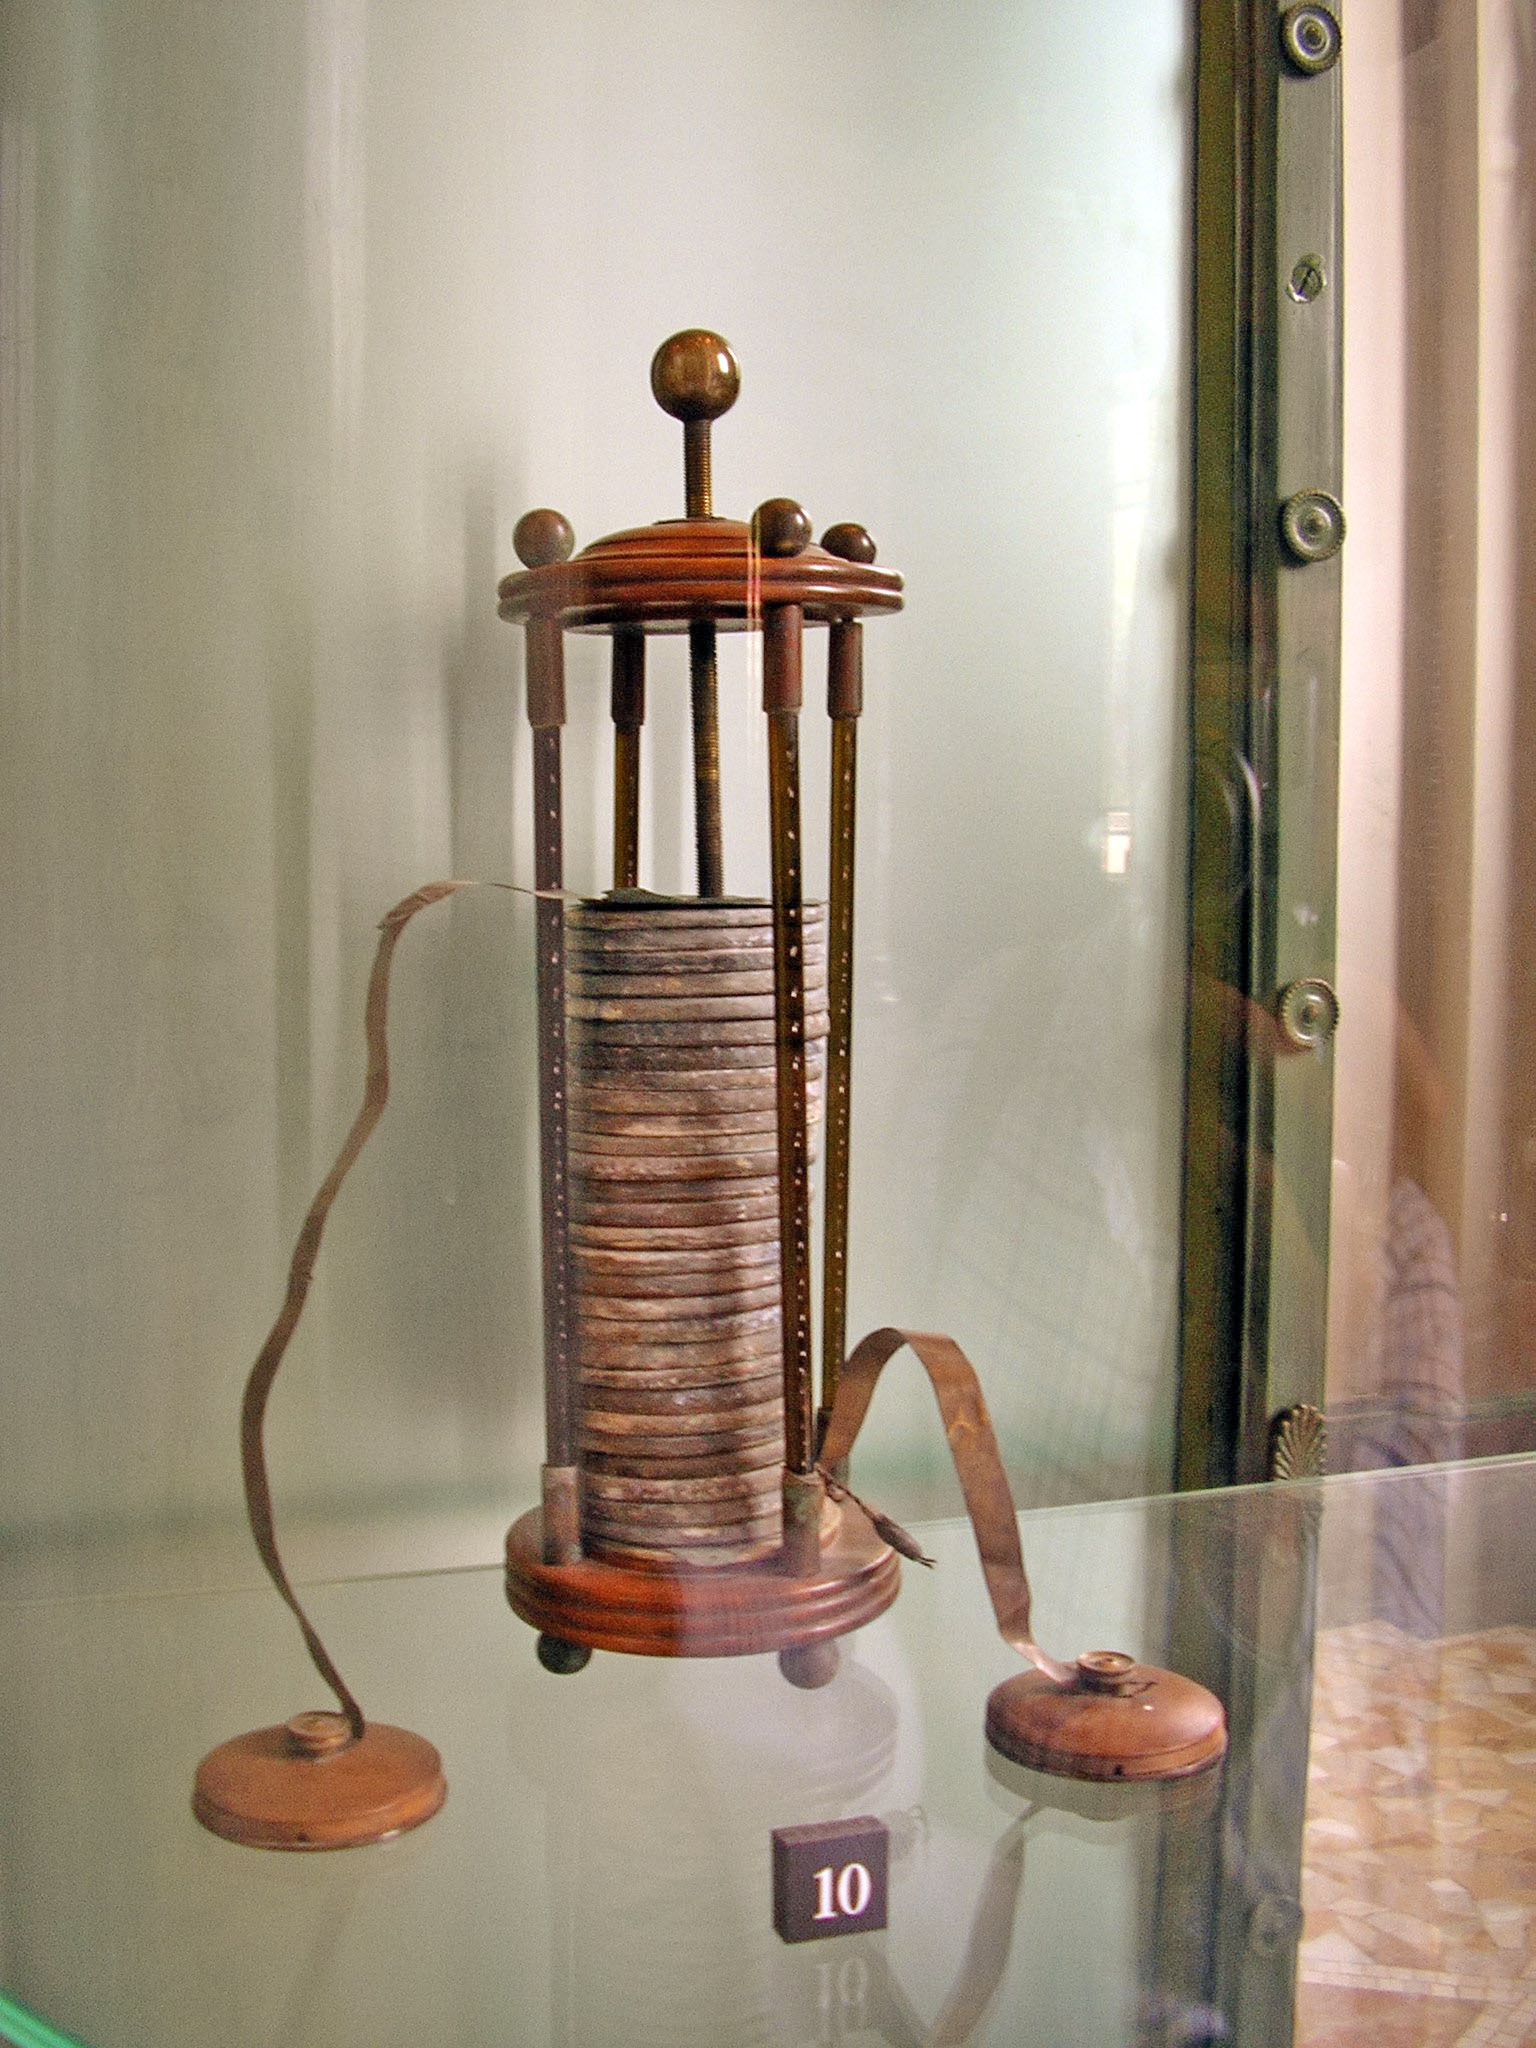
\includegraphics[width=0.24\linewidth]{images/book1/volta-pile.jpg}

{\small Una pila voltaica en un museo. Foto de GuidoB, CC BY-SA 3.0.}
\end{omfigure}

\section{La tensión de una pila}

\begin{definition}[Tensión de una pila]\label{def:g12:cells-and-electrolysis:emf}
La \emph{tensión de una pila}\index{tension de una pila@tensión de una pila} es la tensión
medida con un voltímetro entre los bornes de una pila que no suministra
corriente (en circuito abierto); es positiva cuando el borne positivo del
voltímetro está en el \omterm{def:g12:cells-and-electrolysis:anode}{cátodo}.
\end{definition}

\begin{example}[La pila Daniell]\label{ex:g12:cells-and-electrolysis:daniell}
% ledger: e0:Cu, e0:Zn, emf:Daniell
Con las dos disoluciones a \qty{1}{mol/L}, la pila Daniell da
\qty{1.10}{V}. Cómo se predice esa tensión a partir de tablas de
potenciales de electrodo se muestra en el volumen del primer año.
\end{example}

\begin{remark}[Por qué se gasta una pila]\label{rem:g12:cells-and-electrolysis:runs-down}
La reacción de la pila, \ce{Zn + Cu^{2+} -> Zn^{2+} + Cu}, tiene una
constante $K$ muy grande. Mientras la pila funciona,
$Q = [\ce{Zn^{2+}}]/[\ce{Cu^{2+}}]$ aumenta, y la reacción sigue mientras
$Q < K$. Cuando se agota un \omterm{def:g7:chemical-reactions:reactant}{reactivo} (el cinc, o los \omterm{def:g9:ions:ion}{iones} cobre), la
corriente se detiene: la pila está ``gastada''.
\end{remark}

\section{Carga y capacidad}

\begin{definition}[Constante de Faraday, capacidad]\label{def:g12:cells-and-electrolysis:capacity}
La \emph{constante de Faraday}\index{constante de Faraday} $F$ es la
carga eléctrica de un \omterm{def:g10:the-mole:amount}{mol} de \omterm{def:g9:inside-the-atom:nucleus}{electrones}, $F = N_A e = \qty{96485}{C/mol}$.
La \emph{capacidad}\index{capacidad} de una pila es la mayor carga
eléctrica que puede suministrar, a menudo expresada en amperios hora:
$\qty{1}{A.h} = \qty{3600}{C}$.
\end{definition}

\begin{proposition}[Carga y cantidad de electrones]\label{prop:g12:cells-and-electrolysis:charge}
% ledger: const:F, const:NA, const:e
Una corriente $I$ que circula durante un tiempo $\Delta t$ transporta la
carga $Q = I\,\Delta t$, es decir, una cantidad de \omterm{def:g9:inside-the-atom:nucleus}{electrones}
\[
  n(e^-) = \frac{Q}{F} = \frac{I\,\Delta t}{F} .
\]
\end{proposition}

\begin{proof}
Cada \omterm{def:g9:inside-the-atom:nucleus}{electrón} lleva la carga elemental $e$; $n$ \omterm{def:g10:the-mole:amount}{moles} de \omterm{def:g9:inside-the-atom:nucleus}{electrones}
llevan $n N_A e = n F$.
\end{proof}

\begin{example}[Capacidad de una pila Daniell]\label{ex:g12:cells-and-electrolysis:capacity}
% ledger: aw:Zn, const:F
El electrodo de cinc contiene \qty{6.5}{g} de cinc que puede reaccionar,
es decir, $6.5/65.4 = \qty{0.099}{mol}$. Cada \omterm{def:g7:atoms-and-molecules:atom}{átomo} de cinc cede dos
\omterm{def:g9:inside-the-atom:nucleus}{electrones}: $n(e^-) = \qty{0.199}{mol}$, así que
$Q = 0.199 \times 96485 = \qty{1.9e4}{C}$, unos
$\qty{1.9e4}{}/3600 = \qty{5.3}{A.h}$, si los \omterm{def:g9:ions:ion}{iones} cobre no se agotan
antes.
\end{example}

\section{Electrólisis}

\begin{definition}[Electrólisis, acumulador]\label{def:g12:cells-and-electrolysis:electrolysis}
Una \emph{electrólisis}\index{electrolisis@electrólisis} es una \omterm{def:g11:redox:reaction}{reacción redox} forzada
por un generador eléctrico, en el sentido opuesto al que tomaría por sí
sola. Un \emph{acumulador}\index{acumulador} es una pila que se puede
recargar: durante la carga, el generador la obliga a ir en sentido
inverso, como en una electrólisis.
\end{definition}

\begin{inthelab}[Electrólisis del agua]
Dos electrodos se sumergen en agua que se ha hecho conductora con un poco
de sulfato de sodio, cada uno bajo un tubo de ensayo invertido lleno de
la disolución. Con un generador de unos pocos voltios, suben burbujas de
ambos electrodos: en el \omterm{def:g12:cells-and-electrolysis:anode}{cátodo} (conectado al borne $-$), dihidrógeno; en
el \omterm{def:g12:cells-and-electrolysis:anode}{ánodo}, dioxígeno; del primero se forma el doble que del segundo. Una
astilla encendida produce una pequeña detonación en el primer gas; una
astilla incandescente se reaviva en el segundo.
\end{inthelab}

\begin{omfigure}
\begin{tikzpicture}[font=\small, scale=1.2]
  % a trough of water, two inverted tubes standing in it
  \fill[omWater] (-1.4,0) rectangle (1.4,1.1);
  \foreach \x/\g in {-0.6/1.2, 0.6/0.6} {
    \fill[omWater] (\x-0.18,0.3) rectangle (\x+0.18,2.9);
    \fill[white] (\x-0.18,{2.9-\g}) rectangle (\x+0.18,2.9);
    \fill[white] (\x,2.9) circle (0.18);
    \draw[om glass] (\x-0.18,0.3) -- (\x-0.18,2.9) arc[start angle=180, end angle=0, radius=0.18] -- (\x+0.18,0.3);
  }
  \draw[om glass] (-1.5,1.25) -- (-1.4,1.15) -- (-1.4,0) -- (1.4,0) -- (1.4,1.15) -- (1.5,1.25);
  \fill[black!55] (-0.65,0) rectangle (-0.55,0.6);
  \fill[black!55] (0.55,0) rectangle (0.65,0.6);
  \node[draw, fill=white, minimum width=1.6cm, minimum height=0.45cm, font=\footnotesize] (g) at (0,-0.75) {generador};
  \draw[black!70, thick] (-0.6,0) -- (-0.6,0 |- g.north);
  \draw[black!70, thick] (0.6,0) -- (0.6,0 |- g.north);
  \node[font=\footnotesize] at (-0.78,-0.3) {$-$};
  \node[font=\footnotesize] at (0.78,-0.3) {$+$};
  \node[anchor=east, align=right] at (-0.95,2.5) {dihidrógeno\\ (cátodo)};
  \node[anchor=west, align=left] at (0.95,2.5) {dioxígeno\\ (ánodo)};
\end{tikzpicture}

{\small \omterm{def:g12:cells-and-electrolysis:electrolysis}{Electrólisis} del agua: sobre los electrodos se recoge el doble de
dihidrógeno que de dioxígeno.}
\end{omfigure}


\begin{example}[El agua, descompuesta]\label{ex:g12:cells-and-electrolysis:water}
En el \omterm{def:g12:cells-and-electrolysis:anode}{cátodo}: \ce{2H2O + 2e- -> H2 + 2OH-}; en el \omterm{def:g12:cells-and-electrolysis:anode}{ánodo}:
\ce{6H2O -> O2 + 4H3O+ + 4e-}. Por cada cuatro \omterm{def:g9:inside-the-atom:nucleus}{electrones}, dos \omterm{def:g7:atoms-and-molecules:molecule}{moléculas}
de dihidrógeno y una de dioxígeno, mientras que los \omterm{def:g9:ions:ion}{iones} \ce{H3O+} y
\ce{OH-} formados en los dos electrodos se recombinan en agua: en
conjunto, \ce{2H2O -> 2H2 + O2}, la
inversa de la \omterm{def:g4:what-a-fire-needs:burning}{combustión} del hidrógeno, que necesita energía para
producirse.
\end{example}

\begin{method}[Masa depositada por una electrólisis]\label{met:g12:cells-and-electrolysis:mass}
\begin{enumerate}
  \item Escribe la \omterm{def:g11:redox:couple}{semiecuación} en el electrodo donde se forma el \omterm{def:g9:periodic-table-first-look:metal}{metal},
        por ejemplo \ce{Cu^{2+} + 2e- -> Cu}.
  \item Calcula la carga $Q = I \Delta t$ y $n(e^-) = Q/F$.
  \item Divide por el número de \omterm{def:g9:inside-the-atom:nucleus}{electrones} por \omterm{def:g7:atoms-and-molecules:atom}{átomo}: $n(\ce{Cu}) =
        n(e^-)/2$; después, $m = n \times M$.
\end{enumerate}
\end{method}


\begin{example}[El refinado del cobre]\label{ex:g12:cells-and-electrolysis:refining}
% ledger: aw:Cu, const:F
El cobre impuro que sale de la fundición se usa como \omterm{def:g12:cells-and-electrolysis:anode}{ánodo} de una cuba
de \omterm{def:g12:cells-and-electrolysis:electrolysis}{electrólisis} con disolución de sulfato de cobre, y una lámina fina de
cobre puro como \omterm{def:g12:cells-and-electrolysis:anode}{cátodo}. En el \omterm{def:g12:cells-and-electrolysis:anode}{ánodo}, el cobre se \omterm{def:g2:mixing-and-dissolving:dissolve}{disuelve},
\ce{Cu -> Cu^{2+} + 2e-}; en el \omterm{def:g12:cells-and-electrolysis:anode}{cátodo} se deposita cobre puro,
\ce{Cu^{2+} + 2e- -> Cu}; las impurezas caen al fondo o se quedan en
disolución. Una corriente de \qty{100}{A} durante \qty{24}{h} transporta
$Q = 100 \times 86400 = \qty{8.64e6}{C}$, es decir,
$n(e^-) = \qty{89.5}{mol}$, que depositan $89.5/2 = \qty{44.8}{mol}$ de
cobre: \qty{2.84}{kg}.
\end{example}

\begin{omfigure}
\begin{tikzpicture}[font=\small, scale=1.25]
  \pic[transform shape] at (0,0) {beaker={0.75}{cyan!70!blue!35}};
  \pic[transform shape] (an) at (-0.4,0.2) {electrode={orange!40!brown!80!black}};
  \pic[transform shape] (ca) at (0.4,0.2) {electrode={orange!80!brown}};
  \foreach \p in {(-0.6,0.08),(-0.5,0.12),(-0.3,0.07),(-0.2,0.1)} \fill[black!55] \p circle (0.03);
  \node[draw, fill=white, font=\footnotesize, minimum width=1.6cm] (g) at (0,3.4) {generador};
  \draw[black!70, thick] (an-top) -- (an-top |- g.south);
  \draw[black!70, thick] (ca-top) -- (ca-top |- g.south);
  \node[font=\footnotesize] at (-0.58,2.95) {$+$};
  \node[font=\footnotesize] at (0.58,2.95) {$-$};
  \draw[omProp, thick, <-] (-0.55,1.2) -- (-1.6,1.6) node[left, align=right, text=black] {ánodo de cobre\\ impuro: se disuelve};
  \draw[omProp, thick, <-] (0.55,1.2) -- (1.6,1.6) node[right, align=left, text=black] {cátodo de cobre\\ puro: crece};
  \draw[omProp, thick, <-] (-0.35,0.1) -- (-1.6,0.3) node[left, text=black] {impurezas};
\end{tikzpicture}

{\small Refinado del cobre por \omterm{def:g12:cells-and-electrolysis:electrolysis}{electrólisis}: el cobre pasa del \omterm{def:g12:cells-and-electrolysis:anode}{ánodo}
impuro al \omterm{def:g12:cells-and-electrolysis:anode}{cátodo} puro a través de la disolución.}
\end{omfigure}

\section{Pilas, acumuladores y pilas de combustible}

Toda pila desechable es una \omterm{def:g12:cells-and-electrolysis:cell}{pila electroquímica}, y toda batería
recargable, un \omterm{def:g12:cells-and-electrolysis:electrolysis}{acumulador}. El \omterm{def:g12:cells-and-electrolysis:electrolysis}{acumulador} de plomo de un coche funciona
con plomo, óxido de plomo y ácido sulfúrico; el \omterm{def:g12:cells-and-electrolysis:electrolysis}{acumulador} de ion-litio
de un teléfono desplaza \omterm{def:g9:ions:ion}{iones} litio entre dos electrodos, uno de grafito
y otro de un óxido metálico, a través de un electrolito líquido o
polimérico, mientras los \omterm{def:g9:inside-the-atom:nucleus}{electrones} recorren el circuito exterior. Una
pila de \omterm{def:g4:what-a-fire-needs:fuel}{combustible} es una pila cuyos \omterm{def:g7:chemical-reactions:reactant}{reactivos} se suministran de forma
continua: una pila de \omterm{def:g4:what-a-fire-needs:fuel}{combustible} de hidrógeno lleva a cabo la reacción
\ce{2H2 + O2 -> 2H2O}, la inversa de la \omterm{def:g12:cells-and-electrolysis:electrolysis}{electrólisis} del agua, y da
electricidad y agua. El dihidrógeno obtenido por \omterm{def:g12:cells-and-electrolysis:electrolysis}{electrólisis} con
electricidad eólica o solar, y usado después en pilas de \omterm{def:g4:what-a-fire-needs:fuel}{combustible}, es
una forma de almacenar esa electricidad.

\begin{omfigure}
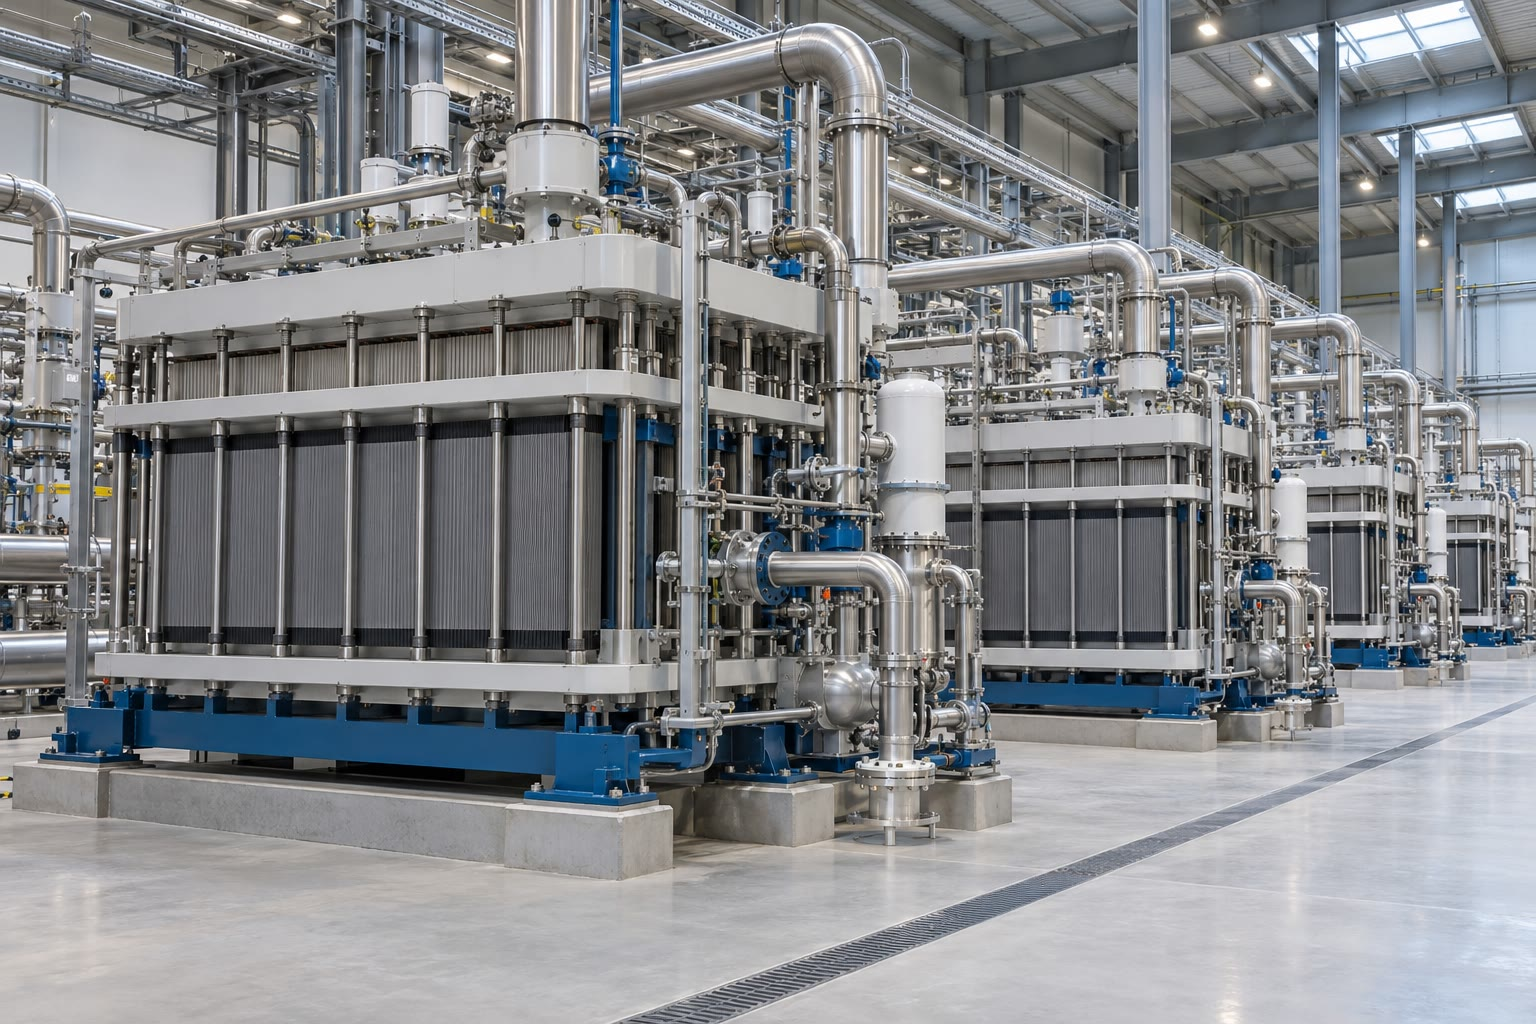
\includegraphics[width=0.48\linewidth]{images/book1/ai/g12-electrolyser-hall.jpg}

{\small Una nave de electrolizadores: el agua se descompone en
dihidrógeno y dioxígeno.}
\end{omfigure}

\section{Ejercicios}

\begin{exercise}[$\star$]\label{exo:g12:cells-and-electrolysis:1}
En la pila Daniell, ¿qué electrodo es el \omterm{def:g12:cells-and-electrolysis:anode}{ánodo}? ¿Y el \omterm{def:g12:cells-and-electrolysis:anode}{cátodo}? Escribe la
\omterm{def:g11:redox:couple}{semiecuación} en cada uno.
\end{exercise}

\begin{exercise}[$\star$]\label{exo:g12:cells-and-electrolysis:2}
Una corriente de \qty{0.20}{A} circula durante \qty{30}{min}. Calcula la
carga transportada y la cantidad de \omterm{def:g9:inside-the-atom:nucleus}{electrones}.
\end{exercise}

\begin{exercise}[$\star$]\label{exo:g12:cells-and-electrolysis:3}
¿Cuál es el papel del \omterm{def:g12:cells-and-electrolysis:cell}{puente salino}? ¿Qué ocurre si se retira?
\end{exercise}

\begin{exercise}[$\star$]\label{exo:g12:cells-and-electrolysis:4}
Convierte una \omterm{def:g12:cells-and-electrolysis:capacity}{capacidad} de \qty{2.5}{A.h} en culombios.
\end{exercise}

\begin{exercise}[$\star$]\label{exo:g12:cells-and-electrolysis:5}
En una \omterm{def:g12:cells-and-electrolysis:electrolysis}{electrólisis}, ¿es espontánea la reacción? ¿Qué aporta la energía?
\end{exercise}

\begin{exercise}[$\star\star$]\label{exo:g12:cells-and-electrolysis:6}
Una pila está formada por un electrodo de plata en nitrato de plata y un
electrodo de cobre en sulfato de cobre. El voltímetro muestra que los
\omterm{def:g9:inside-the-atom:nucleus}{electrones} salen por el cobre. Escribe las \omterm{def:g11:redox:couple}{semiecuaciones}, nombra el
\omterm{def:g12:cells-and-electrolysis:anode}{ánodo} y el \omterm{def:g12:cells-and-electrolysis:anode}{cátodo}, y da la reacción global.
\end{exercise}

\begin{exercise}[$\star\star$]\label{exo:g12:cells-and-electrolysis:7}
La pila de un reloj suministra \qty{10}{\micro A} de forma continua
durante tres años. ¿Cuál es su \omterm{def:g12:cells-and-electrolysis:capacity}{capacidad} en \si{mA.h}?
\end{exercise}

\begin{exercise}[$\star\star$]\label{exo:g12:cells-and-electrolysis:8}
Una cuchara se platea con una corriente de \qty{0.50}{A} durante
\qty{40}{min}, \ce{Ag+ + e- -> Ag}. ¿Qué masa de plata se deposita?
\end{exercise}

\begin{exercise}[$\star\star$]\label{exo:g12:cells-and-electrolysis:9}
En la figura de la pila Daniell, da el sentido de la corriente en el
cable y el sentido en el que se desplazan los \omterm{def:g9:ions:ion}{iones} \ce{K+} y \ce{NO3-}
del puente.
\end{exercise}

\begin{exercise}[$\star\star$]\label{exo:g12:cells-and-electrolysis:10}
Compara una pila y una \omterm{def:g12:cells-and-electrolysis:electrolysis}{electrólisis}: el signo del \omterm{def:g12:cells-and-electrolysis:anode}{ánodo}, el sentido de la
reacción y la conversión de energía.
\end{exercise}

\begin{exercise}[$\star\star$]\label{exo:g12:cells-and-electrolysis:11}
En la \omterm{def:g12:cells-and-electrolysis:electrolysis}{electrólisis} del agua se recogen \qty{24}{mL} de dihidrógeno. ¿Qué
volumen de dioxígeno se recoge al mismo tiempo? ¿Por qué?
\end{exercise}

\begin{exercise}[$\star\star\star$]\label{exo:g12:cells-and-electrolysis:12}
Una pila Daniell contiene \qty{5.0}{g} de cinc y \qty{100}{mL} de sulfato
de cobre a \qty{0.50}{mol/L}. ¿Qué \omterm{def:g7:chemical-reactions:reactant}{reactivo} se agota primero? ¿Cuál es la
\omterm{def:g12:cells-and-electrolysis:capacity}{capacidad} de la pila? ¿Durante cuánto tiempo puede suministrar
\qty{50}{mA}?
\end{exercise}

\begin{exercise}[$\star\star\star$]\label{exo:g12:cells-and-electrolysis:13}
Una pila de \qty{1.5}{V} suministra \qty{2.0}{A.h}. Calcula la energía
que almacena ($E = Q U$), en julios y en vatios hora.
\end{exercise}

\begin{exercise}[$\star\star\star$]\label{exo:g12:cells-and-electrolysis:14}
Se electroliza agua con \qty{2.0}{A} durante \qty{1.0}{h}. Calcula las
cantidades, y después los volúmenes a \qty{20}{\celsius}
($V_m = \qty{24.1}{L/mol}$), de dihidrógeno y de dioxígeno producidos.
\end{exercise}

\begin{exercise}[$\star\star\star$]\label{exo:g12:cells-and-electrolysis:15}
En el refinado del cobre, el \omterm{def:g12:cells-and-electrolysis:anode}{ánodo} pierde \qty{3.00}{kg} de material
mientras el \omterm{def:g12:cells-and-electrolysis:anode}{cátodo} gana \qty{2.84}{kg} de cobre. ¿Cuál es el porcentaje
de cobre del \omterm{def:g12:cells-and-electrolysis:anode}{ánodo} impuro, suponiendo que en el \omterm{def:g12:cells-and-electrolysis:anode}{ánodo} solo se oxida el
cobre y que las impurezas simplemente se desprenden?
\end{exercise}

\section{Problema: la batería del teléfono}

\begin{problem}[{Problema de fin de semana --- ¿qué masa de litio va y viene entre
los electrodos de una batería de teléfono de \qty{4000}{mA.h}?}]
\label{pb:g12:cells-and-electrolysis:1}
% ledger: const:F, const:NA, aw:Li, dch:CH4, aw:C, aw:H
La batería de un teléfono lleva la indicación ``\qty{3.7}{V},
\qty{4000}{mA.h}''. En una imagen simplificada, durante la descarga cada
\omterm{def:g7:atoms-and-molecules:atom}{átomo} de litio almacenado en el electrodo de grafito cede un \omterm{def:g9:inside-the-atom:nucleus}{electrón} y
sale como \omterm{def:g9:ions:ion}{ion} litio, \ce{Li -> Li+ + e-}; el \omterm{def:g9:ions:ion}{ion} atraviesa el electrolito
y lo capta el electrodo de óxido metálico, que gana un \omterm{def:g9:inside-the-atom:nucleus}{electrón} al mismo
tiempo.

\medskip
\noindent\textbf{Parte I --- La pila.}
\begin{enumerate}
  \item Durante la descarga, ¿el electrodo de grafito es el \omterm{def:g12:cells-and-electrolysis:anode}{ánodo} o el
        \omterm{def:g12:cells-and-electrolysis:anode}{cátodo}? ¿Por qué?
  \item ¿Cuál es el polo negativo?
  \item ¿En qué sentido viajan los \omterm{def:g9:inside-the-atom:nucleus}{electrones} a través del teléfono? ¿Y
        los \omterm{def:g9:ions:ion}{iones} litio dentro de la batería?
  \item ¿Por qué esta pila es un \omterm{def:g12:cells-and-electrolysis:electrolysis}{acumulador}?
\end{enumerate}

\medskip
\noindent\textbf{Parte II --- La carga.}
\begin{enumerate}[resume]
  \item Convierte \qty{4000}{mA.h} en amperios hora, y después en
        culombios.
  \item Calcula la cantidad de \omterm{def:g9:inside-the-atom:nucleus}{electrones} que representa esta carga.
  \item ¿Cuántos \omterm{def:g9:inside-the-atom:nucleus}{electrones} son?
  \item El teléfono consume en promedio \qty{0.25}{A}. ¿Cuánto dura una
        batería llena?
  \item La pantalla muestra un 20 \%. ¿Qué carga, en culombios, queda?
\end{enumerate}

\medskip
\noindent\textbf{Parte III --- La energía.}
\begin{enumerate}[resume]
  \item Calcula la energía almacenada, $E = Q U$, en julios.
  \item Conviértela en vatios hora.
  \item Compárala con la energía liberada al quemar \qty{1}{g} de metano
        (\qty{55.7}{kJ}).
  \item ¿Cuántas cargas completas da \qty{1}{kW.h} de electricidad, si no
        se perdiera energía?
\end{enumerate}

\medskip
\noindent\textbf{Parte IV --- La recarga.}
\begin{enumerate}[resume]
  \item Durante la carga, ¿qué reacción tiene lugar en el electrodo de
        grafito? ¿Es una \omterm{def:g11:redox:oxidation}{oxidación} o una \omterm{def:g11:redox:oxidation}{reducción}?
  \item ¿Por qué la recarga es una \omterm{def:g12:cells-and-electrolysis:electrolysis}{electrólisis}?
  \item El cargador suministra \qty{2.0}{A}. ¿Cuánto tarda como mínimo una
        recarga completa?
  \item ¿Qué cantidad de \omterm{def:g9:ions:ion}{iones} litio atraviesa el electrolito durante una
        carga completa?
  \item Calcula su masa.
  \item Da la respuesta final: ¿qué masa de litio va y viene entre los
        electrodos en una carga completa?
\end{enumerate}
\end{problem}
